\chapter{Ricerca}
\section{Ricerca e protocollo}

L’interesse per le relazioni tra occhio, postura e apparato stomatognatico sta crescendo, come dimostra la letteratura
scientifica dell’ultimo decennio e l’approccio dei clinici a riguardo. In particolare le ricerche riportano la presenza di
un’associazione clinica tra le malocclusioni dentali e i difetti di convergenza, come descritto da Silverstrini-Biavati et al. 9
Bilello et al. hanno condotto uno studio che ha portato a verificare la correlazione tra sistema stomatognatico e
oculomotore, notando la presenza di eteroforie o eterotropie e difetti di convergenza in persone con malocclusioni
dentali 10 . Un’altra ricerca condotta da Monaco ed al. suggerisce la correlazione tra difetti di refrazione e malocclusioni,
in particolare: l’incidenza di astigmatismo e ipermetropia è maggiore in soggetti con prima classe dentaria, mentre la
miopia è maggiore per soggetti con seconda classe 11 .

In seguito alla lettura di questi studi e all’approfondimento delle connessioni nervose presenti tra i due sistemi, è nata
l’idea di questa ricerca. Essa propone di verificare il cambiamento del sistema visivo in seguito al trattamento
logopedico e osteopatico dell’apparato stomatognatico in soggetti con disfunzioni primarie orofacciali. Ciò che si vuole
verificare è che la riabilitazione delle disfunzioni orofacciali porti a un miglioramento dei difetti visivi della persona. Per
difetto visivo si intende: anomalie refrattive, accomodative, muscolari, di convergenza e stabilità. Lo svolgimento della
ricerca è stato effettuato a Brescia presso il negozio di ottica Ottico Bertella e in collaborazione con l’ambulatorio della
dottoressa Alice Delbono (logopedista) e il dottor Stefano Grassotti (osteopata, fisioterapista), nei mesi da settembre
2016 a gennaio 2017. Sono stati coinvolti tutti i soggetti affluenti presso l’ambulatorio e i conoscenti della laureanda e
dei collaboratori, per un totale di 93 persone. Tra questi sono stati selezionati complessivamente 19 soggetti che
rispettavano i criteri di inclusione e si sono rivelati disponibili alla partecipazione e all’impegno. Questi sono stati divisi
in gruppo sperimentale e gruppo di controllo in base alle scelte dei singoli.

\section{Materiali e metodi}

Sono stati selezionati 19 soggetti con primarietà deglutitoria e squilibrio muscolare oro-facciale di età media di 25 anni:
10 appartenenti al gruppo sperimentale, 9 appartenenti al gruppo di controllo. Sono stati esclusi:

\begin{itemize}
 \itemsep-0.5em
 \item[--]Soggetti con terapia logopedica per la rieducazione della deglutizione in corso
 \item[--]Soggetti con malattie neurodegenerative
 \item[--]Soggetti non collaboranti (deficit cognitivi, bambini sotto i 6 anni)
\end{itemize}

Entrambi i gruppi sono stati sottoposti ad una valutazione osteopatica-posturale iniziale, dove si è risaliti alla
disfunzione primaria linguale e deglutitoria. Si parla di disfunzione primaria linguale e deglutitoria quando l’alterazione
della funzione linguale genera la disfunzione di altri recettori del STP a cascata, per motivi prevalentemente neurologici
(connessioni tra nuclei della base dei diversi nervi cranici, in particolare III, IV, V, VI, XI nervi cranici).

Successivamente ciascun soggetto è stato valutato dal punto di vista optometrico. La valutazione è stata ripetuta a
distanza di tre mesi per il gruppo di controllo e prima e dopo il trattamento logopedico-osteopatico di tre mesi per il
gruppo sperimentale. Essa comprendeva i seguenti test:

\begin{itemize}
 \itemsep-0.5em
 \item[--]Refrazione
 \item[--]Stereopsi lontano e vicino
 \item[--]Foria ambientale lontano, con il metodo di Howell
 \item[--]Punto prossimo di convergenza effettuato nelle posizioni: diritto, basso e alto
 \item[--]Foria ambientale da vicino con il metodo di Howell, effettuato nelle posizioni: diritto, basso, alto
 \item[--]Cover test nelle 9 posizioni di sguardo con quantificazione con prismi
 \item[--]Ampiezza accomodativa tramite metodo push up
 \item[--]Disparità di fissazione con Wesson Card
 \item[--]MEM
 \end{itemize}
 

\subsection{Svolgimento della ricerca}

\subsubsection{Test posturali per stabilire primarietà linguale}
\\\
I test posturali esplorano i riflessi neurofisiologici del STP e permettono di ottenere informazioni sul cambiamento
della postura, della simmetria del tono e della forza muscolare, stimolando o inibendo l’attività dei recettori posturali.
A seguito della stimolazione o inibizione può verificarsi il miglioramento o peggioramento della funzione indagata (per
esempio della simmetria del tono muscolare) a seconda di quale recettore viene considerato.

Nella ricerca sono stati utilizzati diversi test posturali, tra cui il “test degli indici” che “studia le simmetrie del tono
muscolare attraverso modificazioni delle informazioni recettoriali” 12 Si inizia proponendo il test di base posizionando il
soggetto in stazione eretta con denti non a contatto e piedi in posizione neutra. Si chiede quindi di anteporre gli arti
superiori con gli indici in avanti. L’arto più indietreggiato segnala un aumento omolaterale del tono dei muscoli
estensori della colonna vertebrale. Dopo aver eseguito il test di base si verifica l’adattamento fra i diversi recettori e il
sistema tonico posturale in vari modi, ad esempio:
\begin{itemize}
 \itemsep-0.5em
 \item[--]si chiede di guardare a destra e a sinistra per attivare la muscolatura estrinseca oculare e il sistema oculogiro. In
fisiologia eseguendo questo test si ha un aumento del tono muscolare contro laterale con arretramento dell’arto. Ad
esempio: la rotazione degli occhi a sinistra fa aumentare il tono dei muscoli estensori di destra, quindi arretra l’arto
superiore di destra. Se ciò non avviene si rileva un problema di oculomotricità non adattato dal STP, quindi il risultato
del test si definisce positivo.
 \item[--]si chiede al soggetto di protrudere la lingua e di deviarla a destra e a sinistra per valutare la risposta del STP rispetto al
recettore linguale. Ad esempio se in un soggetto, quando protrude la lingua, il test di base risulta modificato significa
che vi è una probabile disfunzione linguale che interferisce sul STP, quindi il risultato del test è positivo.
\end{itemize}

Al termine della valutazione si possono osservare diversi risultati positivi, ad esempio in un soggetto si può trovare una
positività sia al test del sistema oculogiro che al test del recettore linguale. Diventa necessario quindi stabilire quale sia
il recettore che interferisce maggiormente con il STP (disfunzione primaria) e che porta in disfunzione anche l’altro
recettore (disfunzione secondaria).

Un recettore risulta primario se, dopo averlo stimolato, porta ad un miglioramento degli altri recettori. Ad esempio se
si ha sia positività del recettore oculare sia positività del recettore linguale si può effettuare uno stretching della lingua
e, in seguito, verificare con il test degli indici se i test descritti sopra sono diventati negativi. Se ciò avviene si ha una
primarietà linguale e la disfunzione del recettore oculare risulta secondaria alla disfunzione linguale. Se invece dopo lo
stretching linguale il test sul recettore linguale risulta negativo a occhi chiusi mentre positivo ad occhi aperti, allora la
disfunzione del recettore oculare è primaria sulla disfunzione linguale.
\\\ \\\
\subsubsection{Test per visita optometrica}
\\\ 
Per tutti i test, eccetto la refrazione, è stato utilizzato l’eventuale occhiale che sarebbe stato indossato durante il
periodo di trattamento. Laddove il soggetto avesse cambiato correzione senza preavviso, i test pre e post trattamento
sono stati effettuati con le stesse lenti. Inoltre è stato valutato il grado di fatica (da 1 che indica assenza di fatica a 5 che
indica molta fatica) provato durante lo svolgimento di ogni test.
\\\ \\\
\textbf{Refrazione:} la refrazione è stata effettuata tramite il metodo della sospensione foveale, laddove il soggetto non
presentava fastidi. In alternativa è stato effettuato il test #7 con il forottero. Il risultato riportato è dato dalla lente che
permettesse la migliore acutezza visiva e il migliore bilanciamento binoculare per il soggetto.
\\\ \\\
\textbf{Stereopsi:} è stato utilizzato per vicino il test della mosca di Titmus a 40 cm, in particolare si fa riferimento al test con
cerchi per la percezione della profondità (da 800 a 40 sec).

\begin{figure}[h!]
	\centering
	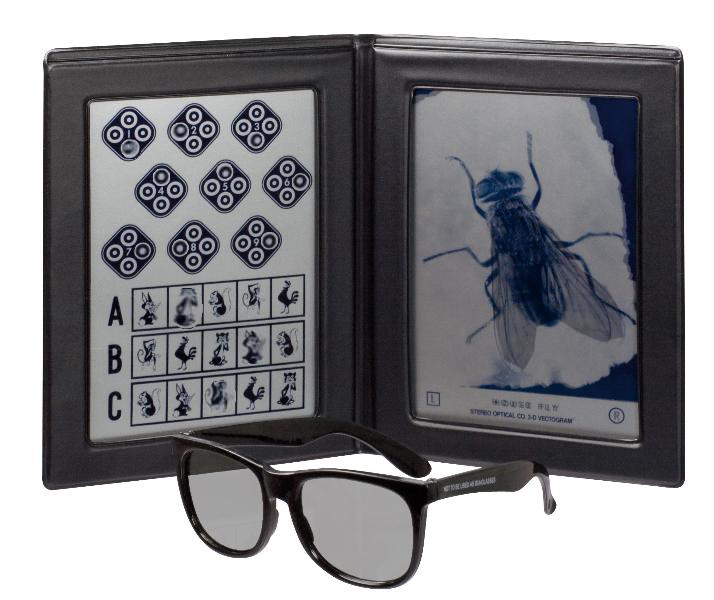
\includegraphics[scale=0.22]{source/immagini/titmus.jpg}
	\caption[Semantic Web stack]{Test Mosca di Titmus}
	\label{fig:issuexample}
\end{figure}

\textbf{Foria ambientale:} lo scopo era di individuare il disallineamento degli assi visivi in condizione di dissociazione da
lontano e vicino. È stata utilizzata la Howell Card a 40 cm, con un prisma di 6\^ base alta. Da vicino si è valutata la foria
in posizione: basso (circa 45\° sotto lo sguardo), diritto, alto (circa 45\° sopra lo sguardo).

\begin{figure}[h!]
\centering
\begin{minipage}{.5\textwidth}
  \centering
  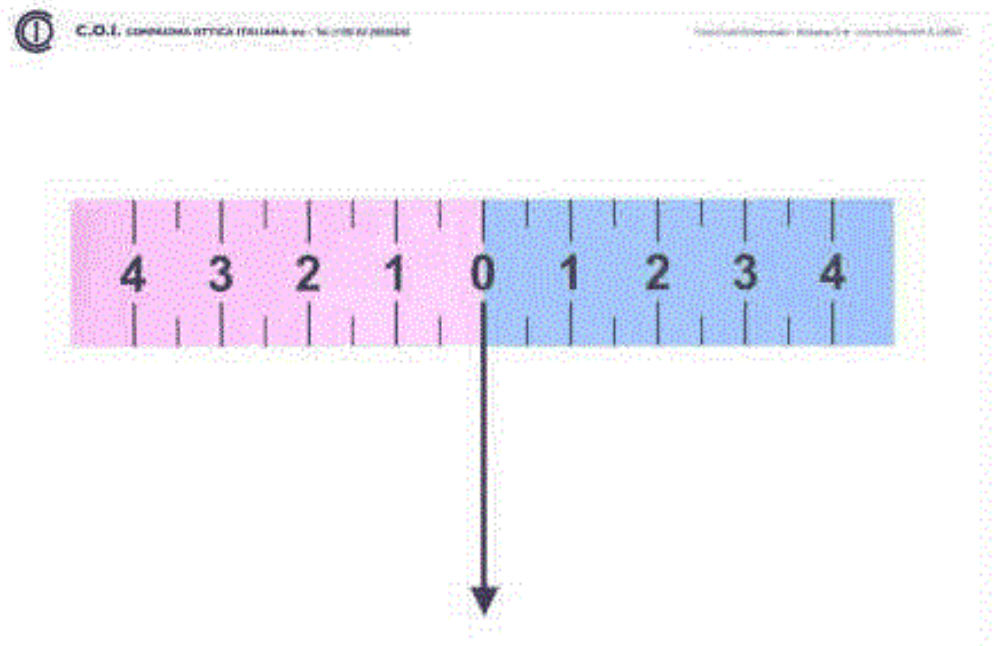
\includegraphics[scale=0.15]{source/immagini/foria_lontano.png}
  \captionof{figure}{Howell card lontano}
  \label{fig:test1}
\end{minipage}%
\begin{minipage}{.5\textwidth}
  \centering
  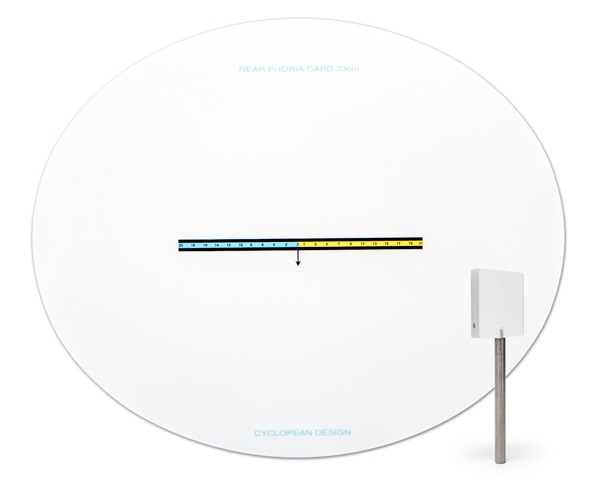
\includegraphics[scale=0.41]{source/immagini/foria_vicino.jpg}
  \captionof{figure}{Howell card vicino}
  \label{fig:test2}
\end{minipage}
\end{figure}
\\\ \\\
\textbf{Punto prossimo di convergenza (PPC):} l’obiettivo era di valutare il punto di rottura e recupero della binocularità del
soggetto, quindi comprendere la sua stabilità e capacità di recupero della binocularità. Si è voluto valutare come
variava il PPC nella posizione in basso, diritto e in alto. É stato utilizzato come target una penlight e si chiedeva di
osservare la luce finché non si fosse sdoppiata e riferire poi quanto tornava singola.
\\\ \\\
\textbf{Cover test:} il test è stato utilizzato per valutare e quantificare in modo oggettivo il funzionamento e la stabilità della
muscolatura estrinseca dell’occhio. È stato effettuato mostrando la penlight ad una distanza di circa 30 cm nelle 9
posizioni di sguardo, seguendo l’H diagnostica, in modo da poter valutare la stabilità conferita dai muscoli oculari.
L’instabilità è stata quantificata con l’utilizzo dei prismi Base Interna per le exoforie/tropie, Base Esterna per le
esoforie/tropie.

\begin{figure}[H]
\centering
\begin{minipage}{.5\textwidth}
  \centering
  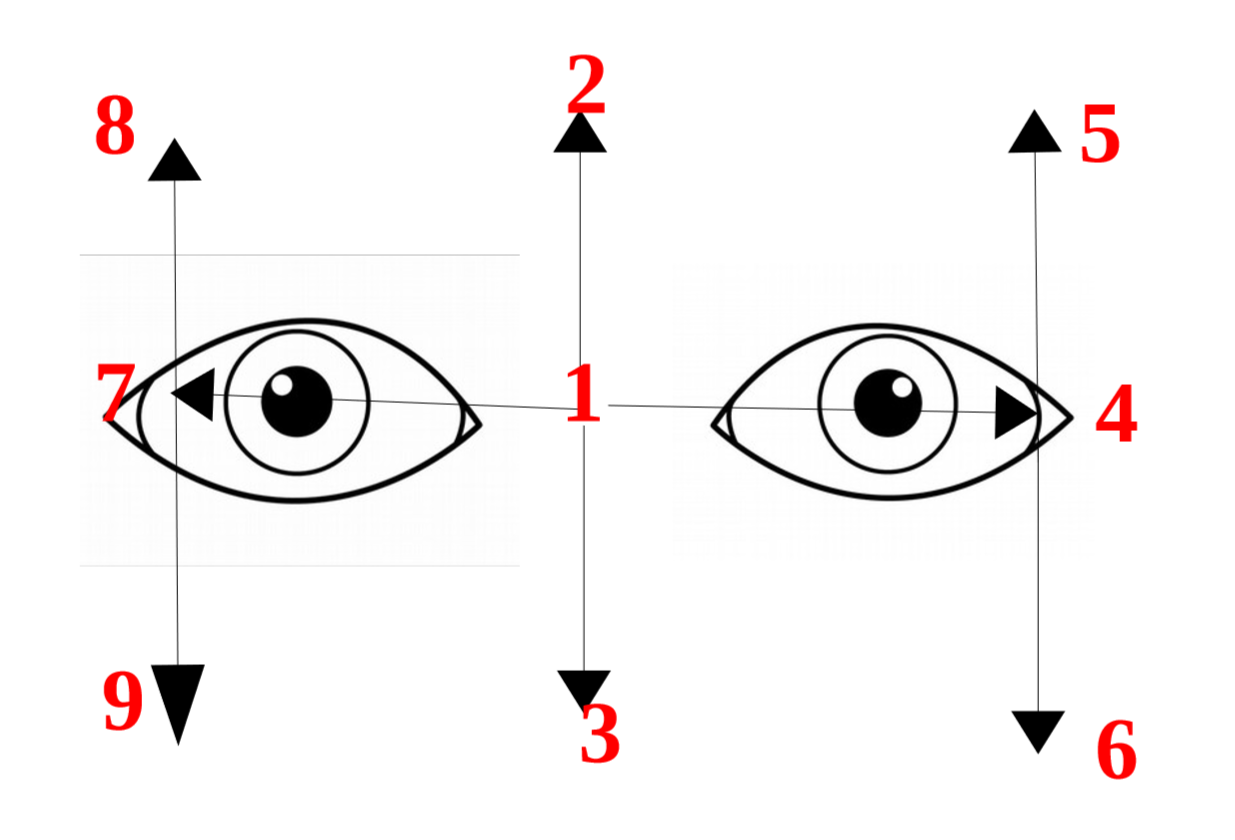
\includegraphics[scale=0.3]{source/immagini/posizioni_cover_test.png}
  \captionof{figure}{Indicazione posizione di sguardo indagate}
  \label{fig:test1}
\end{minipage}%
\begin{minipage}{.5\textwidth}
  \centering
  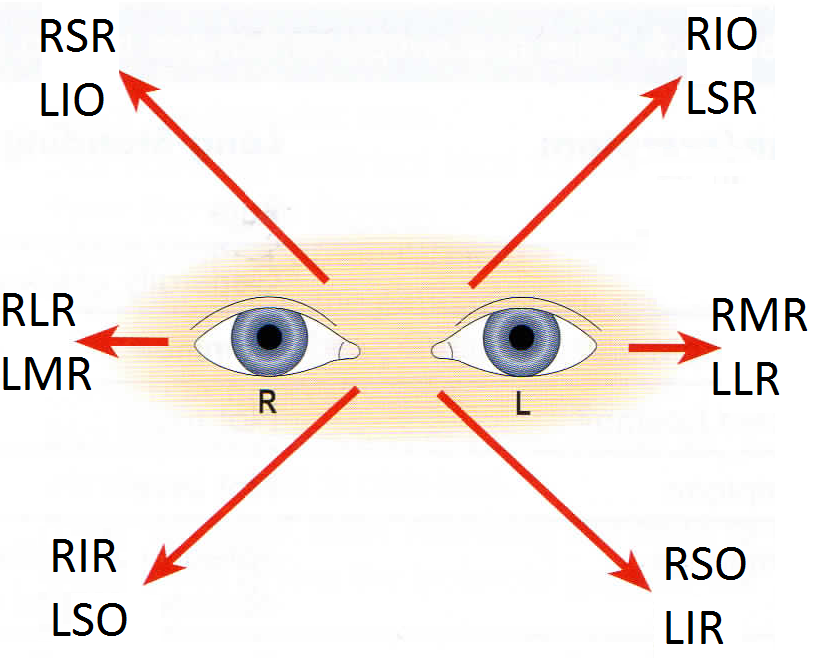
\includegraphics[scale=0.39]{source/immagini/posizioni_di_sguardo.png}
  \captionof{figure}{Muscoli stimolati nelle varie posizioni di sguardo}
  \label{fig:test2}
\end{minipage}
\end{figure}
\\\ \\\
\textbf{Ampiezza Accomodativa:} lo scopo era di valutare la capacità accomodativa del soggetto, tenendo conto dell’età. É stato
utilizzato il metodo Push up per occhio destro, sinistro e binoculare, utilizzando come target i numeri della bacchetta di
Lang e quantificando in centimetri.

\begin{figure}[h!]
	\centering
	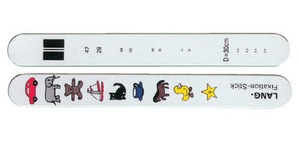
\includegraphics[scale=0.5]{source/immagini/ampiezza_accomodativa.jpg}
	\caption[Semantic Web stack]{Bacchetta di Lang per l'ampiezza accomodativa}
	\label{fig:issuexample}
\end{figure}
\\\ \\\
\textbf{Disparità di fissazione:} utilizzata per valutare la posizione degli assi visivi in condizioni di binocularità. É stata mostrata
la Wesson Card a 25 cm, con occhialini polarizzati e quantificata in minuti d’arco.

\begin{figure}[h!]
	\centering
	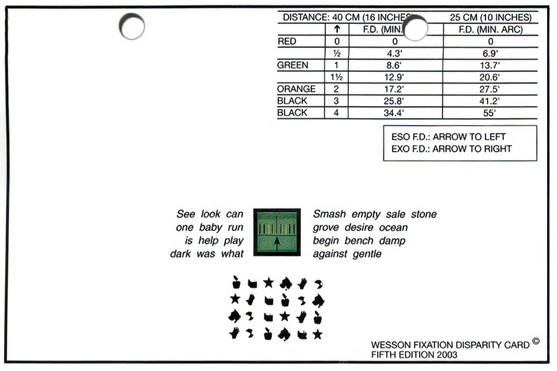
\includegraphics[scale=0.22]{source/immagini/Wesson_card.jpg}
	\caption[Semantic Web stack]{Wesson card}
	\label{fig:issuexample}
\end{figure}
\\\ \\\
\textbf{MEM:} il test è stato effettuato per valutare la posizione del piano accomodativo del soggetto, quantificato con lenti
positive per LAG e negative per LEAD.

\subsubsection{Valutazione e trattamento dello SMOF}

La valutazione del soggetto con squilibrio muscolare orofacciale comprende: 

\begin{enumerate}
\item \textbf{Raccolta anamnestica}
\begin{itemize}
 \item Anamnesi famigliare
 \item Anamnesi fisiologica sono state poste domande su: allattamento, presenza di abitudini viziate e parafunzioni, tipo di alimentazione, atteggiamenti posturali scorretti
  \item Anamnesi patologica si è indagata la presenza di patologie che possono aver facilitato l'esordio di una disfunzione muscolare orofacciale (traumi, carie, deviazioni del setto nasale o polipi nasali, allergie, frequenti infezioni delle vie respiratorie, otiti, perforazioni timpaniche)
\end{itemize}
\item \textbf{Esame obiettivo}, con lo scopo di valutare il tono e la funzione di distretti muscolari (orbicolare delle labbra, mentale, buccinatore, muscoli masticatori, muscoli del pavimento orale, muscoli linguali, nasali, diaframma, muscoli sopraioidei e sottoioidei)
\item \textbf{Analisi delle funzioni} dell'apparato stomatognatico (posizione linguale a riposo, durante l'atto deglutitorio ed in fonazione, masticazione, tipo e modalità di respirazione)
\end{enumerate}

Durante l’esame obiettivo si sono analizzate alcune caratteristiche del soggetto, quali la distanza naso-mento (se varia durante la deglutizione è un indice significativo di deglutizione deviata) e l'angolo cervico-pelvi-mandibolare (se ottuso potrebbe indicare deglutizione deviata).

Moyers distingue due tipi di deglutizione atipica: 
\begin{itemize}
 \itemsep-0.5em
  \item[--]Con  spinta  semplice:  contrazione  dei  muscoli  periorali,  contrazione  degli elevatori mandibolari, spinta linguale anteriore, arcate dentali a contatto
  \item[--]Con  spinta  complessa:  contrazione  dei  muscoli  periorali,  nessuna contrazione degli  elevatori  mandibolari,  spinta  linguale  anteriore  con lingua  e/o  labbro inferiore interposto tra le arcate dentali che non giungono, così, a contatto.
\end{itemize}

\begin{figure}[h!]
	\centering
	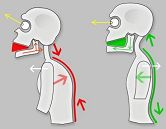
\includegraphics[scale=0.9]{source/immagini/angolo_cervico-pelvi-mandibolare.jpg}
	\caption[Semantic Web stack]{Differenza tra angolo cervico-pelvi-mandibolare ottuso (sinistra) e normale (destra)}
	\label{fig:issuexample}
\end{figure}

\textbf{Piano di trattamento}
\\\
In seguito è stato svolto il trattamento logopedico dello squilibrio muscolare orofacciale che si fonda soprattutto sui principi e sulla pratica della Terapia Miofunzionale. Quest’ultimo è un metodo rieducativo volto al raggiungimento di un equilibrio nel tono dei muscoli oro-facciali e alla correzione delle funzioni di pertinenza stomatognatica, quali la deglutizione, la fonazione, la masticazione e la respirazione. Il termine di “Myofunctional Therapy” (MFT) è stato coniato da Lischer nel 1918 e proposto all'American Society of Orthodontists da Rogers. Questi focalizzò l'attenzione sul ruolo determinante che ha il comportamento neuromuscolare nei confronti dello sviluppo dento-scheletrico e della terapia ortodontica. La stimolazione della muscolatura orofacciale può correggere in parte o completamente alcune dismorfosi dentali. Infatti i muscoli vengono considerati come “apparecchi ortodontici viventi" e vanno pertanto rieducati per stabilizzare e migliorare i risultati che si possono ottenere mediante il trattamento ortodontico.

Il piano terapeutico seguito dai soggetti dello studio è diviso in 3 fasi:
\begin{enumerate}
\item allenamento della muscolatura orofacciale con esercizi di rinforzo/rilassamento e stretching. In questa prima fase si utilizzano strumenti per rinforzare il tono dell’orbicolare delle labbra come nell’ “esercizio del bottone”, in cui il soggetto deve posizionare un bottone legato ad un filo tra denti e labbra e tirarlo, facendo resistenza con le labbra.

\begin{figure}[h!]
	\centering
	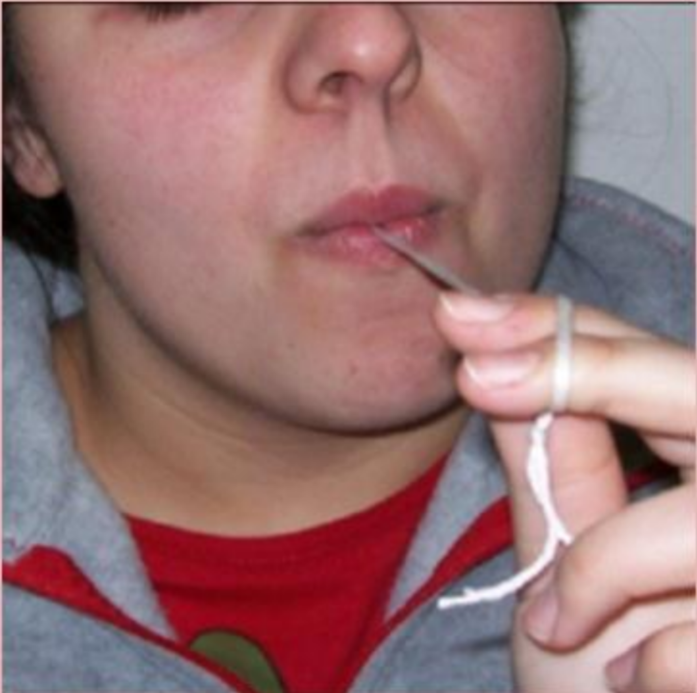
\includegraphics[scale=0.26]{source/immagini/esercizio_del_bottone.png}
	\caption[Semantic Web stack]{Differenza tra angolo cervico-pelvi-mandibolare ottuso (sinistra) e normale (destra)}
	\label{fig:issuexample}
\end{figure}
 
Vengono proposti inoltre esercizi per allenare la postura linguale corretta, per esempio posizionando sull’apice della lingua un elastico ortodontico e chiedendo al soggetto di raggiungere e comprimere lo spot. Questo esercizio è utile anche per allenare l’atto deglutitorio corretto.

\begin{figure}[h!]
\centering
\begin{minipage}{.5\textwidth}
  \centering
  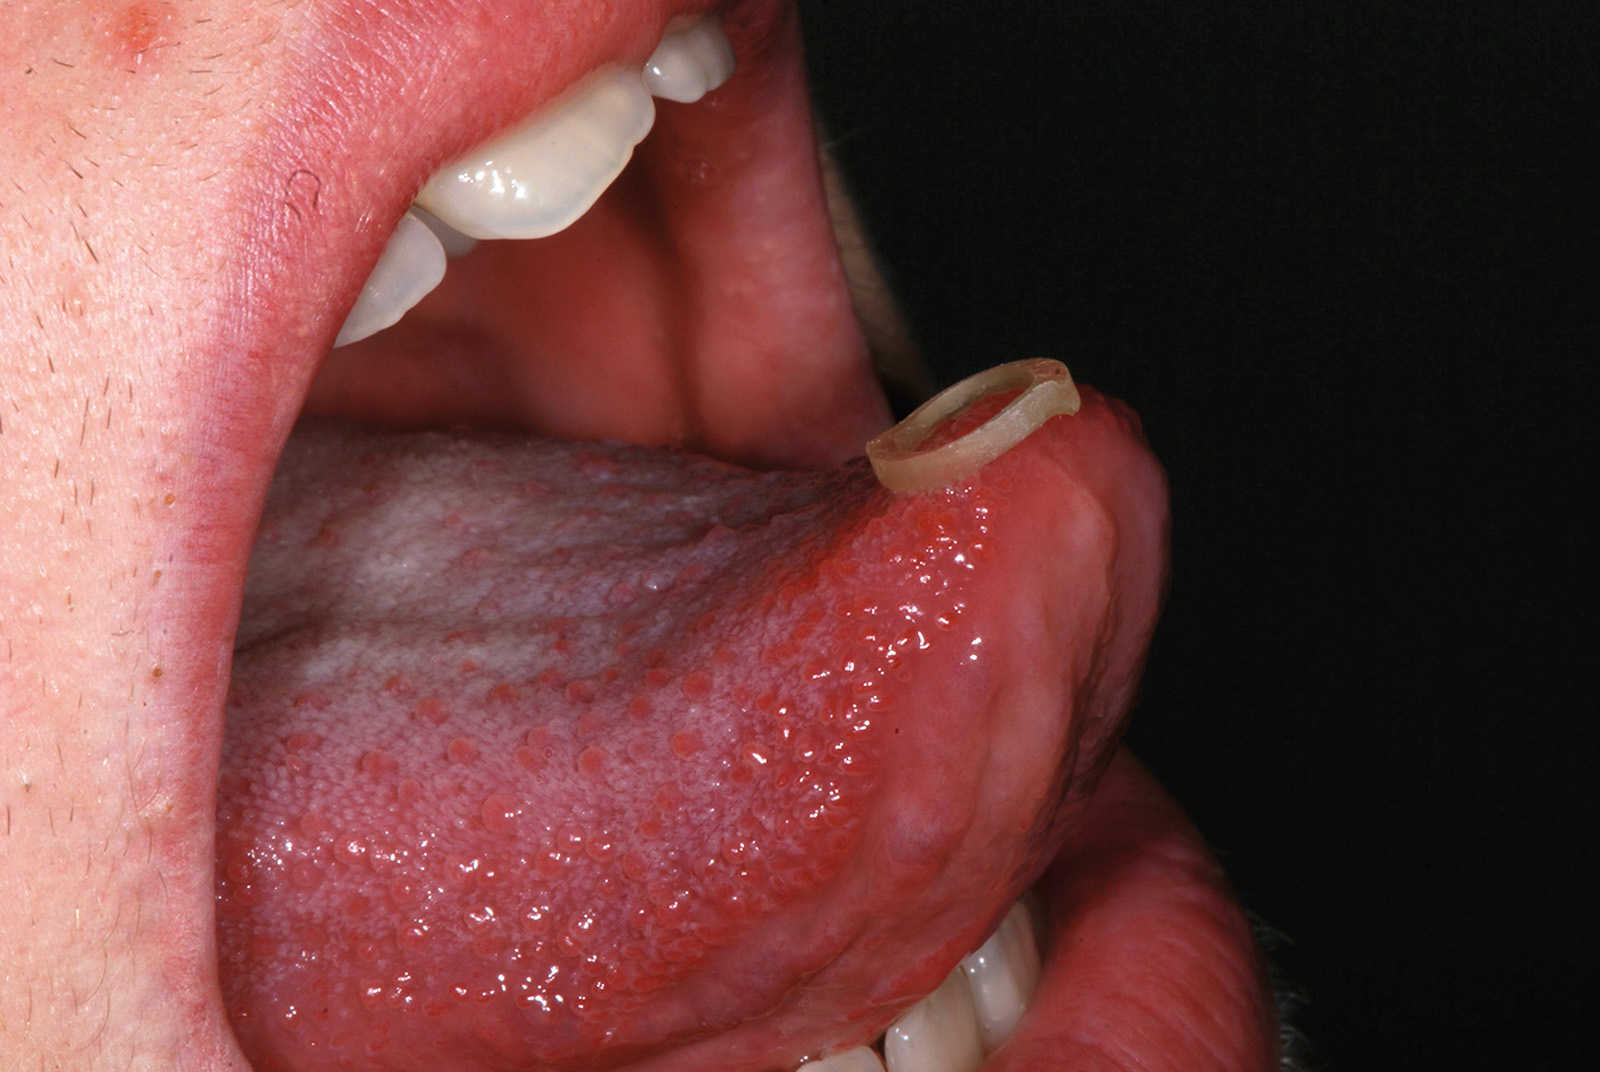
\includegraphics[scale=0.3]{source/immagini/esercizio_spot_fase_1.jpg}
  \captionof{figure}{Indicazione posizione di sguardo indagate}
  \label{fig:test1}
\end{minipage}%
\begin{minipage}{.5\textwidth}
  \centering
  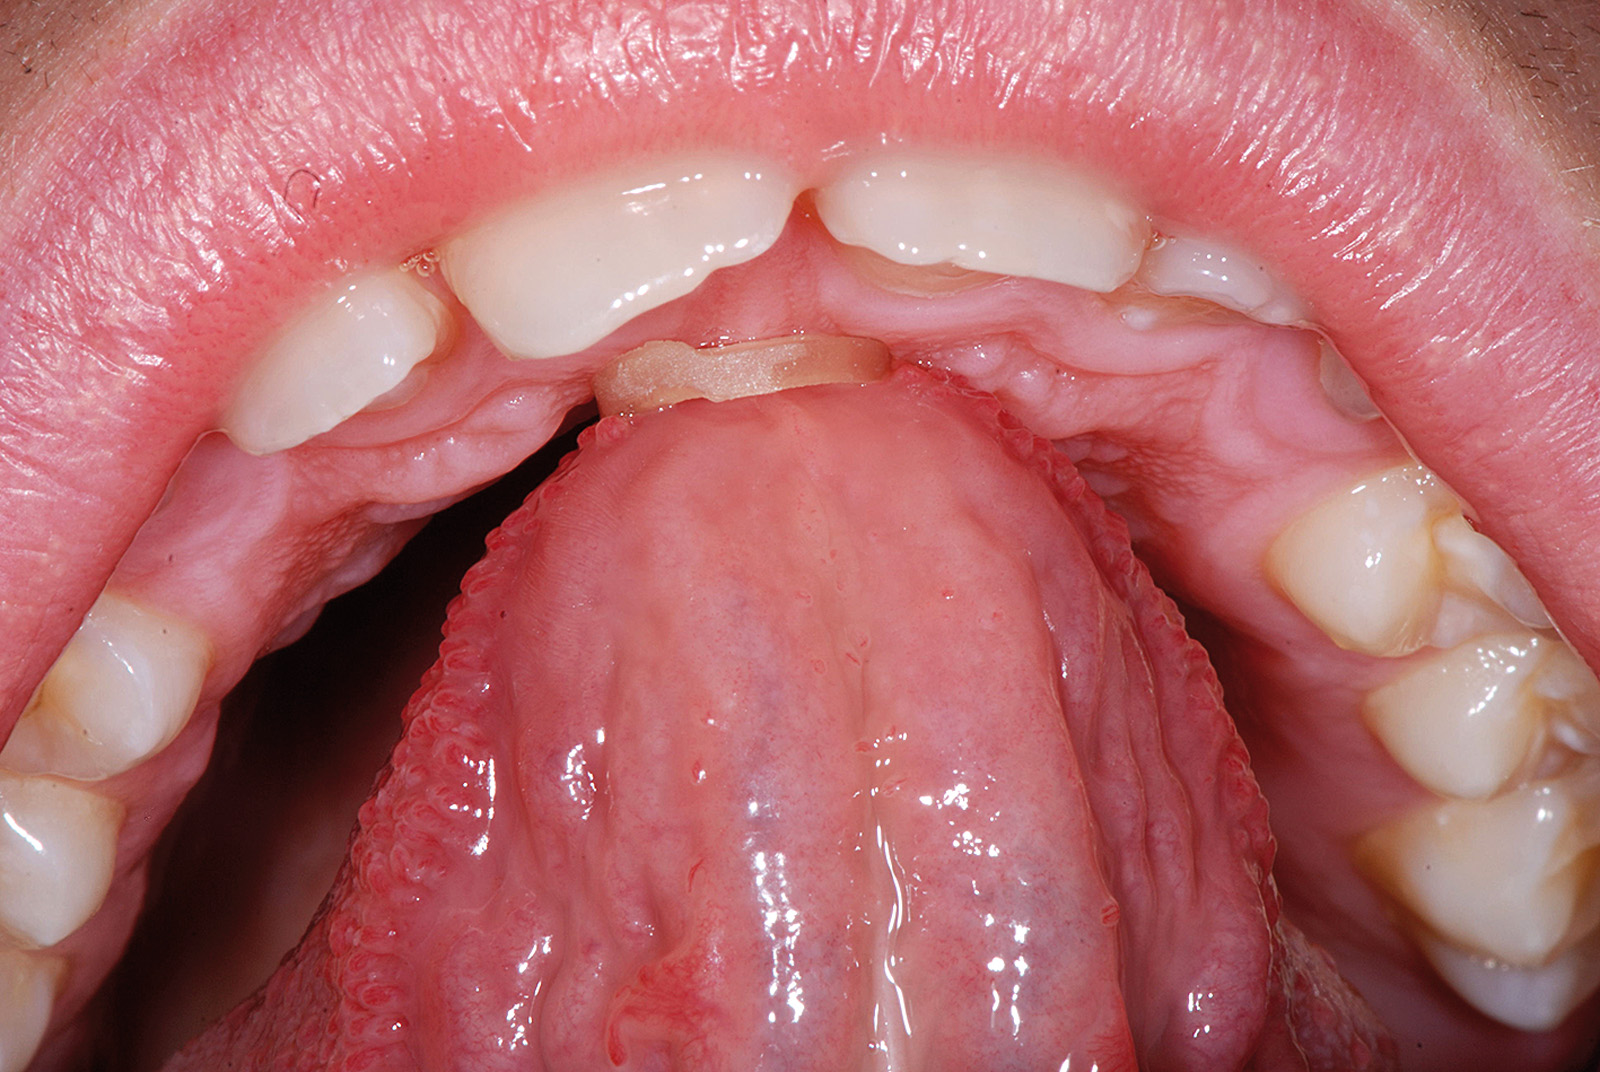
\includegraphics[scale=0.3]{source/immagini/esercizio_spot_fase_2.jpg}
  \captionof{figure}{Muscoli stimolati nelle varie posizioni di sguardo}
  \label{fig:test2}
\end{minipage}
\end{figure}

Gli esercizi vanno eseguiti dal soggetto anche a domicilio almeno una volta al giorno, annotando su una griglia fornita dalla logopedista le sessioni di esercizi eseguite quotidianamente.
\item si insegna al soggetto a deglutire utilizzando cibi solidi e liquidi. Questa fase necessita di maggiore impegno da parte del soggetto, perché durante il pasto deve porre spesso attenzione a come posiziona la lingua mentre sta masticando e deglutendo.
\item si effettuano controlli periodici per verificare se gli esercizi vengono eseguiti correttamente e se l’atto deglutitorio e la postura linguale vengono automatizzati in modo corretto.
\end{enumerate}

Gli esercizi sono stati integrati con il trattamento osteopatico, il quale prevede un approccio globale ed uno locale. Il trattamento globale è stato indirizzato a correggere le disfunzioni più severe e strutturate valutate sul soggetto, interessanti l’apparato muscolo scheletrico e viscerale. Normalizzate queste, si passa ad un approccio mirato al distretto cefalico e alle strutture più intimamente correlate all’apparato stomatognatico dal punto di vista neurologico e tissutale. Si sono valutati e trattati specificamente le articolazioni della base e della volta cranica, il massiccio facciale, i muscoli masticatori, i muscoli sub-occipitali, muscoli sopra e sotto ioidei, il diaframma toracico.



\section{Analisi Statistica}

Per l’analisi statistica dei dati è stato utilizzato il software Libre Office Calc. È stata effettuata sia un’analisi descrittiva dei dati che un’analisi inferenziale. La prima parte mostra la descrizione del campione, la seconda parte riporta i dati in forma grafica confrontando le differenze presenti tra prima e seconda valutazione e tra trattati e non trattati per i test che hanno riportato cambiamenti più evidenti dei valori medi. È stata effettuata anche l’analisi inferenziale tramite il test di Wilcoxon, nonostante la bassa numerosità del campione. Però è proprio grazie al piccolo campione che si è potuta effettuare l’analisi dei singoli dati riscontrati. Infine sono descritti due casi clinici a titolo esemplificativo per testimoniare il cambiamento avvenuto in seguito al trattamento.

\subsection{Analisi descrittive del campione}

I 19 soggetti rientrati nello studio sono stati divisi in 10 nel gruppo sperimentale e in 9 nel gruppo di controllo. Dei 10 soggetti del gruppo sperimentale 7 sono di sesso femminile e 3 di sesso maschile e il 50\% dei soggetti ha un’età inferiore o pari a 22 anni. Dei 9 soggetti del gruppo di controllo 4 sono di sesso femminile e 5 di sesso maschile e il 50\% dei soggetti ha un’età inferiore o pari a 22 anni. Di seguito è riportata una sintesi delle caratteristiche dei soggetti che hanno partecipato alla ricerca:

\begin{table}[H]
\begin{center}
\begin{tabular}{|c|c|c|c|} \hline
{\textbf{}} & {\textbf{Maschio}} & {\textbf{Femmina}}& {\textbf{Totale}}\\ \hline
\textbf{Numero} & 8 & 11 & 19 \\ 
\textbf{Età} & 20.13 & 25.82 & \\ 
\textbf{Min.} & 10 & 12 &  \\ 
\textbf{Max.} & 31 & 55 &\\ 
\textbf{Dev. Std.} & 6.13 & 13.04 &\\

\hline
\end{tabular}
\end{center}
\caption{Dati a confronto dei tre casi considerati}
\end{table}


\begin{table}[H]
\begin{center}
\begin{tabular}{|c|c|c|c|} \hline
{\textbf{}} & {\textbf{Trattati}} & {\textbf{Non trattati}}& {\textbf{Totale}}\\ \hline
\textbf{Maschio} & 3 & 5 & 8 \\
\textbf{Femmina} & 7 & 14 & 11\\ 
\textbf{Totale} & 10 & 9 & 19 \\ 
\textbf{Età} & 25.10 & 21.56 &\\ 
\textbf{Dev. Std.} & 14.52 & 4.42 &\\
\textbf{Mediana} & 22 & 22 &\\

\hline
\end{tabular}
\end{center}
\caption{Dati a confronto dei tre casi considerati}
\end{table}

Di seguito è stato riportato il calcolo e l’analisi dei valori medi del campione sperimentale.

La Tabella 3.3 riporta i valori di media, mediana e moda per tutti i test effettuati, confrontando i dati della prima valutazione (medie 1, mediane 1, mode 1) con i dati della seconda valutazione (medie 2, mediane 2, mode 2) per i soggetti sottoposti al trattamento.


\begin{table}[H]
\begin{center}
\begin{tabular}{|c|c|c|c|c|c|c|} \hline
{\textbf{}} & {\textbf{Medie 1}} & {\textbf{Medie 2}}& {\textbf{Mediane 1}} & {\textbf{Mediane 2}} & {\textbf{Mode 1}} & {\textbf{Mode 2}}\\ \hline
\textbf{Sfero OD} & -0.05 & -0.40 & 0.13 & 0.00 & 0.00 & 0.00 \\ \hline
\textbf{Cilindro OD} & -0.45 & -0.35 & 0.00 & 0.00 & 0.00 & 0.00 \\ \hline
\textbf{Sfero OS} & -0.20 & -0.35 & 0.13 & 0.00 & 0.00 & 0.00 \\ \hline
\textbf{Cilindro OS} & -0.43 & -0.33 & 0.00 & 0.00 & 0.00 & 0.00 \\ \hline
\textbf{Foria L} & 0.00 & 0.05 & 0.00 & 0.25 & 0.00 & 0.50 \\ \hline
\textbf{Stereo L} & 184.00 & 190.00 & 30.00 & 30.00 & 30.00 & 30.00 \\ \hline
\textbf{PPC diritto} & 9.60 & 4.30 & 5.50 & 5.00 & 3.00 & 0.00 \\ \hline
\textbf{PPC alto} & 10.70 & 9.10 & 6.00 & 6.00 & 6.00 & 0.00\\ \hline
\textbf{PPC basso} & 7.80 & 1.10 & 0.50 & 0.00 & 0.00 & 0.00 \\ \hline
\textbf{Foria V alto} & 2.50 & 3.35 & 2.00 & 1.50 & 2.00 & 0.50 \\ \hline
\textbf{Foria V diritto} & 1.90 & 2.35 & 1.50 & 1.50 & 1.00 & 1.00 \\ \hline
\textbf{Foria V basso} & 2.65 & 2.10 & 2.00 & 1.50 & 2.00 & 1.00 \\ \hline
\textbf{CT 1} & 7.40 & 6.60 & 7.00 & 6.50 & 2.00 & 6.00 \\ \hline
\textbf{CT 2} & 10.30 & 11.80 & 12.00 & 11.00 & 0.00 & 8.00\\ \hline
\textbf{CT 3} & 3.30 & 3.40 & 0.00 & 2.00 & 0.00 & 0.00 \\ \hline
\textbf{CT 4} & 5.40 & 5.90 & 3.50 & 4.00 & 0.00 & 4.00 \\ \hline
\textbf{CT 5} & 10.10 & 11.90 & 9.50 & 9.00 & 0.00 & 8.00 \\ \hline
\textbf{CT 6} & 5.00 & 3.20 & 3.00 & 2.00 & 0.00 & 0.00 \\ \hline
\textbf{CT 7} & 11.70 & 7.00 & 8.50 & 6.00 & 0.00 & 6.00 \\ \hline
\textbf{CT 8} & 14.10 & 9.60 & 12.00 & 8.00 & 0.00 & 8.00 \\ \hline
\textbf{CT 9} & 3.30 & 6.60 & 0.00 & 5.00 & 0.00 & 4.00 \\ \hline
\textbf{AA OD} & 8.70 & 10.20 & 8.00 & 9.00 & 4.00 & 6.00 \\ \hline
\textbf{AA OS} & 11.00 & 10.70 & 8.50 & 8.50 & 8.00 & 5.00 \\ \hline
\textbf{AA OO} & 8.00 & 8.90 & 7.00 & 7.00 & 8.00 & 5.00\\ \hline
\textbf{Stereo V} & 138.00 & 44.00 & 70.00 & 40.00 & 40.00 & 40.00\\ \hline
\textbf{DF} & 19.51 & 15.11 & 13.70 & 13.70 & 6.90 & 13.70 \\ \hline
\textbf{MEM OD} & 0.85 & 0.88 & 1.00 & 1.00 & 1.00 & 1.25 \\ \hline
\textbf{MEM OS} & 0.95 & 0.78 & 0.88 & 0.88 & 0.75 & 0.25 \\ \hline

\hline
\end{tabular}
\end{center}
\caption{Valori medi del campione sperimentale}
\end{table}

I dati che devono essere confrontati sono i valori della mediana, la quale ci informa che il 50\% dei soggetti ha presentato un dato non superiore al suo valore. La ricerca si pone di osservare un miglioramento dei valori della seconda valutazione rispetto a quelli della prima. Per miglioramento si intende una riduzione del valore, il quale dovrebbe avvicinarsi allo 0, quindi la differenza tra i dati pre e post trattamento deve essere maggiore di 0. Osservando la variazione della mediana quindi si può supporre che almeno la metà dei soggetti abbia riportato una riduzione del valore e quindi un miglioramento. I seguenti test riportano la presenza di un cambiamento positivo nella mediana almeno di 0,50 unità:

\begin{itemize}
 \itemsep-0.5em
 \item[--]Punto prossimo di convergenza diritto e basso
 \item[--]Foria vicino alto e basso
 \item[--]Cover test in posizione 1 (diritto, nessun muscolo stimolato)
 \item[--]Cover test in posizione  2 (alto in centro; stimolazione: retti superiori entrambi gli occhi)
 \item[--]Cover test in posizione 5 (in alto a sinistra; stimolazione: retto superiore OS, obliquo inferiore OD)
 \item[--]Cover test in posizione  6 (in basso a sinistra; muscoli stimolati: obliquo superiore destro e retto inferiore sinistro)
 \item[--]Cover test in posizione 7 (a destra; muscoli stimolati: retto esterno destro, retto mediale sinistro)
 \item[--]Cover test in posizione 8 (in alto a destra; muscoli stimolati: retto superiore destro, obliquo inferiore sinistro).
 \item[--]Stereopsi vicino
\end{itemize}
\\\
I test che hanno riportato un minimo cambiamento positivo (0,25 unità) o nullo sono:
\begin{itemize}
 \itemsep-0.5em
 \item[--]cilindro e sfero
 \item[--]Foria lontano
 \item[--]Stereopsi lontano
 \item[--]PPC alto
 \item[--]Foria vicino diritto
 \item[--]Ampiezza accomodativa OS
 \end{itemize}
\\\
I test che hanno riportato un peggioramento sono:
\begin{itemize}
 \itemsep-0.5em
 \item[--]Cover test in posizione 3 (in basso al centro; stimolazione: retti inferiori entrambi gli occhi)
 \item[--]Cover test in posizione 4 (a sinistra; stimolazione: retto laterale OS, retto mediale OD)
 \item[--]Cover test in posizione 9 (in basso a destra; stimolazione: obliquo superiore OS, retto inferiore OD)
 \item[--]Ampiezza accomodativa OD e binoculare
 \item[--]Disparità di fissazione
 \item[--]MEM
 \end{itemize}
 
 
 
\subsection{Analisi e discussione dei dati}
 
In questa sezione verrà verificato se è possibile riscontrare un cambiamento statisticamente significativo tra gli esiti dei test effettuati prima e dopo il trattamento logopedico-osteopatico, utilizzando il test di Wilcoxon.
 
In particolare verranno analizzati i test: PPC diritto, CT in posizione 7, CT in posizione 8 e Stereopsi vicino. Questi sono infatti i test che hanno riportato un maggiore miglioramento dei valori medi, quindi si va ad osservare se esso può anche essere considerato statisticamente significativo. Il confronto statistico tra i dati della prima visita e della seconda valutazione è stato misurato utilizzando il test di Wilcoxon (Wilcoxon paired-sample test), il quale si applica nel confronto di dati appaiati quando la variabile in esame non è distribuita in maniera normale. Essa è l’equivalente per dati appaiati del test di Student e può essere effettuato anche per piccoli campioni. L’ipotesi nulla afferma che non ci sia stato alcun cambiamento tra il prima e dopo il trattamento. Il livello di significatività è stato posto a 0.05 e il test è a due code. Si considerano i valori della prima valutazione appaiati con quelli della seconda valutazione. In appendice sono riportati i dati ottenuti dalle valutazioni, calcolando la differenza tra pre e post trattamento. Se la differenza è positiva allora è stato riscontrato un miglioramento, se è pari a 0 allora la condizione è rimasta invariata, se è negativa significa peggioramento.
 
 
 
\subsubsection{Punto prossimo di convergenza (PPC) diritto}

Nella tabella 2 e nella tabella 3 sono mostrati i valori medi dei dati del punto di rottura del PPC in posizione diritta rispettivamente per il gruppo dei trattati e per il gruppo dei non trattati. Nella tabella 4 e 5 sono invece riportati i valori medi dei dati del punto di recupero per, rispettivamente, gruppo dei non trattati e gruppo dei trattati Osservando le tabelle dei dati in appendice, in seguito al trattamento, si nota che nel gruppo sperimentale 5 (50\%) soggetti hanno punti di rottura più vicini, uno (10\%) rimane invariato, mentre 4 (40\%) hanno punti di rottura più distali. 8 (80\%) soggetti invece recuperano a una distanza minore, mentre 2 (20\%) soggetti a distanza maggiore. A distanza di 3 mesi dalla prima visita nel gruppo di controllo si hanno 2 (22,2\%) soggetti che riportano punti di rottura più ravvicinati, 2 (22,2\%) rimangono invariati e 5 (55,5\%) riportano valori più distali. Il punto di recupero per 3 (33,3\%) soggetti del gruppo di controllo è più vicino, 1 (11,1\%) è rimasto invariato mentre per 5 (55,5\%) soggetti è più lontano. 

%%%%%%%%%%%%%%%%%%
\begin{table}
\centering
\setlength\tabcolsep{4pt}
\begin{minipage}{0.48\textwidth}
\centering
\tablewidth=\textwidth

\begin{tabular}{|c|c|c|} \hline
{\textbf{}} & {\textbf{  \hspace{8pt}Prima\hspace{8pt} }} & {\textbf{ \hspace{8pt}Dopo\hspace{8pt}  }}\\ \hline
\textbf{Numeri dati} & 10 & 10 \\ 
\textbf{Media} & 9.60 & 4.30 \\  
\textbf{Dev. Std.} & 11.81 & 3.40 \\  
\textbf{Mediana} & 5.50 & 5.00 \\ 
\textbf{Moda} & 3.00 & 0.00 \\ 
\textbf{Errore Std.} & 12.49 & 3.61 \\ 
\hline
\end{tabular}
\caption{Dati gruppo sperimentale PPC rottura diritto}

\label{tab:accuracy} 
\end{minipage}%
\hfill
\begin{minipage}{0.48\textwidth}
\centering

\begin{tabular}{|c|c|c|} \hline
{\textbf{}} & {\textbf{  \hspace{8pt}Prima\hspace{8pt} }} & {\textbf{ \hspace{8pt}Dopo\hspace{8pt}  }}\\ \hline
\textbf{Numeri dati} & 9 & 9 \\ 
\textbf{Media} & 9.89 & 7.44 \\  
\textbf{Dev. Std.} & 14.28 & 6.54 \\  
\textbf{Mediana} & 6.00 & 5.00 \\  
\textbf{Moda} & 0.00 & \textbackslash \\
\textbf{Errore Std.} & 14.51 & 6.33 \\
\hline
\end{tabular}
\caption{Dati gruppo di controllo PPC rottura diritto}

 \label{tab:ompdiff} 
\end{minipage}
\end{table}
%%%%%%%%%%%%%%%%%%%%%
%%%%%%%%%%%%%%%%%%
\begin{table}
\centering
\setlength\tabcolsep{4pt}
\begin{minipage}{0.48\textwidth}
\centering
\tablewidth=\textwidth

\begin{tabular}{|c|c|c|} \hline
{\textbf{}} & {\textbf{  \hspace{8pt}Prima\hspace{8pt} }} & {\textbf{ \hspace{8pt}Dopo\hspace{8pt}  }}\\ \hline
\textbf{Numeri dati} & 10 & 10 \\
\textbf{Media} & 14.20 & 7.40 \\  
\textbf{Dev. Std.} & 12.32 & 7.72 \\ 
\textbf{Mediana} & 9.00 & 7.00 \\ 
\textbf{Moda} & 8.00 & 0.00 \\ 
\textbf{Errore Std.}& 12.82 & 8.17 \\ 
\hline
\end{tabular}
\caption{Dati gruppo sperimentale PPC recupero diritto}

\label{tab:accuracy} 
\end{minipage}%
\hfill
\begin{minipage}{0.48\textwidth}
\centering

\begin{tabular}{|c|c|c|} \hline
{\textbf{}} & {\textbf{  \hspace{8pt}Prima\hspace{8pt} }} & {\textbf{ \hspace{8pt}Dopo\hspace{8pt}  }}\\ \hline
\textbf{Numeri dati} & 9 & 9 \\ 
\textbf{Media} & 13.56 & 10.33 \\  
\textbf{Dev. Std.} & 16.36 & 7.75 \\  
\textbf{Mediana} & 9.00 & 8.00 \\ 
\textbf{Moda} & 0.00 & 8.00 \\ 
\textbf{Errore Std.} & 16.45 & 7.30\\ 
\hline
\end{tabular}
\caption{Dati gruppo di controllo PPC recupero diritto}

 \label{tab:ompdiff} 
\end{minipage}
\end{table}
%%%%%%%%%%%%%%%%%%%%%
Negli istogrammi sull’asse delle ascisse sono riportati i valori centrali degli intervalli che rappresentano i dati raccolti del punto di rottura/recupero, mentre sull’asse delle ordinate sono presenti le frequenze riscontrate per ogni intervallo. Sono riportati sia il grafico del gruppo sperimentale che quello del gruppo di controllo e le colonne blu si riferiscono ai dati della prima valutazione, mentre quelle rosse ai dati della seconda valutazione.

 \begin{figure}[h!]
	\centering
	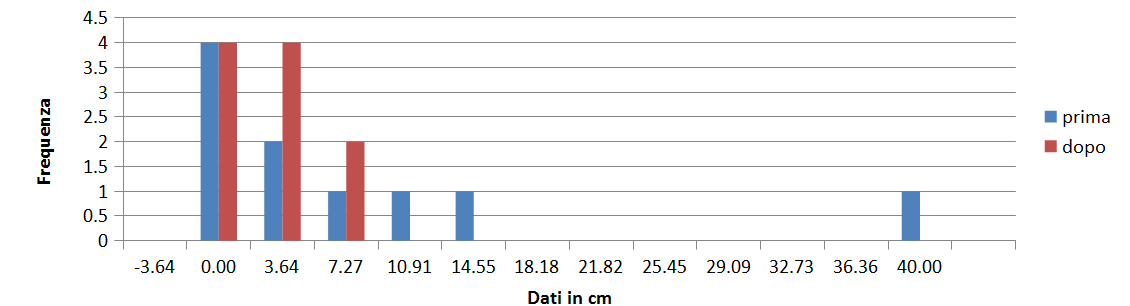
\includegraphics[scale=0.8]{source/grafici/PPC_DIRITTO_DEFINITIVO_sperimentale.png}
	\caption[figure]{Grafico gruppo sperimentale per punto di rottura PPC (diritto): confronto tra prima e seconda valutazione}
	\label{fig:issuexample}
\end{figure}
 \begin{figure}[h!]
	\centering
	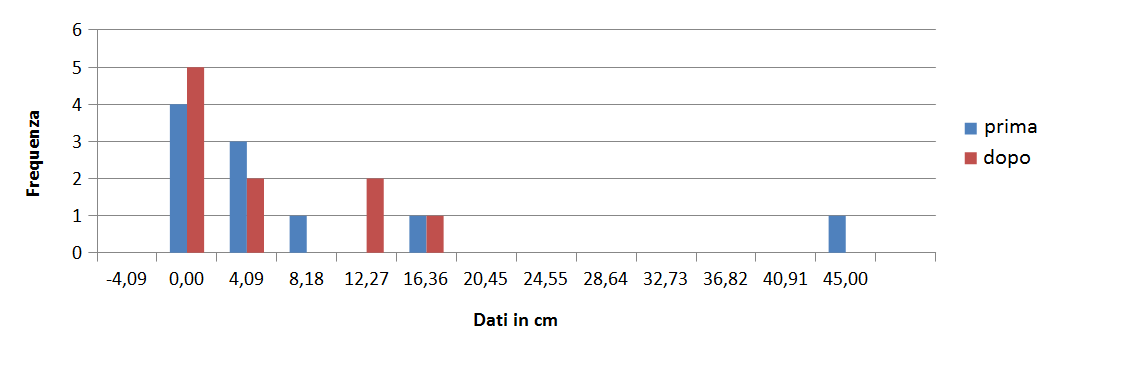
\includegraphics[scale=0.8]{source/grafici/PPC_DIRITTO_DEFINITIVO_GRUPPO_CONTROLLO.png}
	\caption[figure]{Grafico gruppo di controllo per punto di rottura PPC (diritto): confronto tra prima e seconda valutazione}
	\label{fig:issuexample}
\end{figure}
 \begin{figure}[h!]
	\centering
	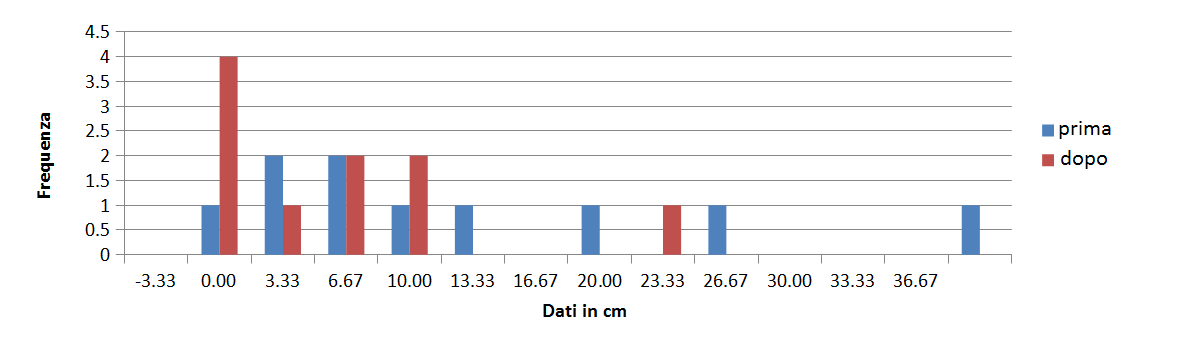
\includegraphics[scale=0.8]{source/grafici/Recupero_PPC_diritto_Trattati.png}
	\caption[figure]{Gruppo sperimentale per punto di recupero PPC (diritto): confronto tra prima e seconda valutazione}
	\label{fig:issuexample}
\end{figure}
 \begin{figure}[h!]
	\centering
	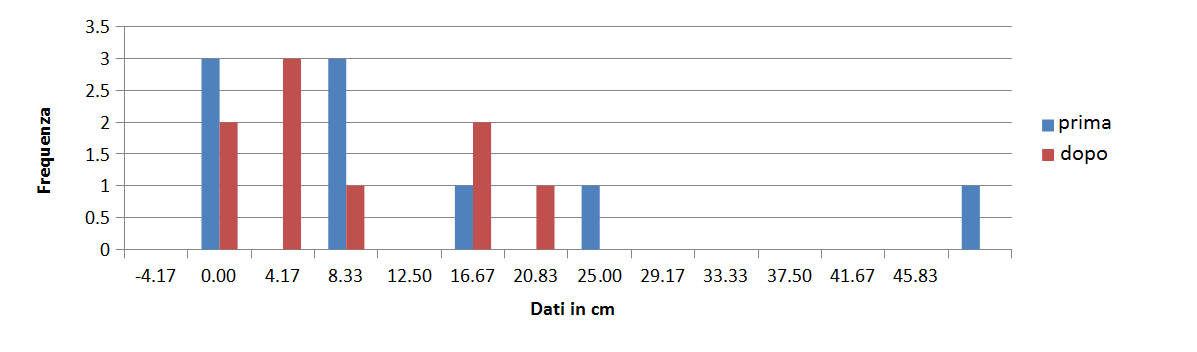
\includegraphics[scale=0.8]{source/grafici/Recupero_PPC_diritto_Non_Trattati.png}
	\caption[figure]{Gruppo di controllo per punto di recupero PPC (diritto): confronto tra prima visita e seconda valutazione}
	\label{fig:issuexample}
\end{figure}

Il test di Wilcoxon riporta per il punto di rottura un W-value di 14.5 il quale, essendo superiore al valore critico (critical value=5), riferisce che il cambiamento non può essere considerato statisticamente significativo. Per il punto di recupero viene riportato un W-value pari a 10.5, con valore critico a 8. Quindi anche per il punto di recupero il cambiamento è non significativo. Osservando però gli istogrammi riportati è possibile notare uno spostamento dei dati verso valori inferiori, quindi con lo spostamento delle colonne rosse verso sinistra. Inoltre dai dati presenti in appendice è possibile notare che un cambiamento è stato effettivamente rilevato, anche se non è stato valutato come statisticamente significativo dal test di Wilcoxon. Infatti il 50\% dei soggetti trattati migliora il valore del punto di rottura e l’80\% riduce il valore del punto di recupero. Al contrario nel gruppo di controllo si riscontra un miglioramento del punto di rottura solo per il 22,2\%, e per il 33,3\% un miglioramento del punto di recupero.


\subsubsection{Cover test in posizione 7}

La posizione 7 corrisponde allo sguardo rivolto a destra, stimolando i muscoli retto esterno dell’occhio destro e il retto interno dell’occhio sinistro. I dati sono stati presi con il valore assoluto, senza considerare se si trattava di eso/exo foria o eso/exo tropia, dal momento che non cambiava l’entità del difetto, ma la sua quantità. In appendice sono riportati i valori e il segno (-) corrisponde a esoforia/tropia, mentre (+) exoforia/tropia. Nel gruppo sperimentale 6 (60\%) soggetti riportano un miglioramento, uno (10\%) rimane invariato e 3 (30\%) sono peggiorati. Nel gruppo di controllo 3 (33,3\%) soggetti riportano un miglioramento, 3 (33,3\%) sono invariati e 3 (33,3\%) sono peggiorati. Nella tabella 6 e 7 vengono inseriti i valori medi del gruppo sperimentale e del gruppo di controllo. Sotto sono riportati gli istogrammi che rappresentano i dati ottenuti nella prima valutazione (colonne blu) e seconda valutazione (colonne rosse).

%%%%%%%%%%%%%%%%%%
\begin{table}
\centering
\setlength\tabcolsep{4pt}
\begin{minipage}{0.48\textwidth}
\centering
\tablewidth=\textwidth

\begin{tabular}{|c|c|c|} \hline
{\textbf{}} & {\textbf{  \hspace{8pt}Prima\hspace{8pt} }} & {\textbf{ \hspace{8pt}Dopo\hspace{8pt}  }}\\ \hline
\textbf{Numeri dati} & 10 & 10 \\ 
\textbf{Media} & 11.70 & 7.00 \\  
\textbf{Dev. Std.} & 14.04 & 4.64 \\  
\textbf{Mediana} & 8.50 & 6.00 \\ 
\textbf{Moda} & 0.00 & 6.00 \\ 
\textbf{Errore Std.} & 14.89 & 4.81 \\ 
\hline
\end{tabular}
\caption{Dati gruppo sperimentale Cover test 7}

\label{tab:accuracy} 
\end{minipage}%
\hfill
\begin{minipage}{0.48\textwidth}
\centering

\begin{tabular}{|c|c|c|} \hline
{\textbf{}} & {\textbf{  \hspace{8pt}Prima\hspace{8pt} }} & {\textbf{ \hspace{8pt}Dopo\hspace{8pt}  }}\\ \hline
\textbf{Numeri dati} & 9 & 9 \\ 
\textbf{Media} & 10.78 & 10.00 \\  
\textbf{Dev. Std.} & 4.41 & 3.46 \\  
\textbf{Mediana} & 12.00 & 8.00 \\  
\textbf{Moda} & 12.00 & 8.00 \\
\textbf{Errore Std.} & 3.84 & 3.70 \\
\hline
\end{tabular}
\caption{Dati gruppo di controllo Cover test 7}

 \label{tab:ompdiff} 
\end{minipage}
\end{table}
%%%%%%%%%%%%%%%%%%%%%
 \begin{figure}[h!]
	\centering
	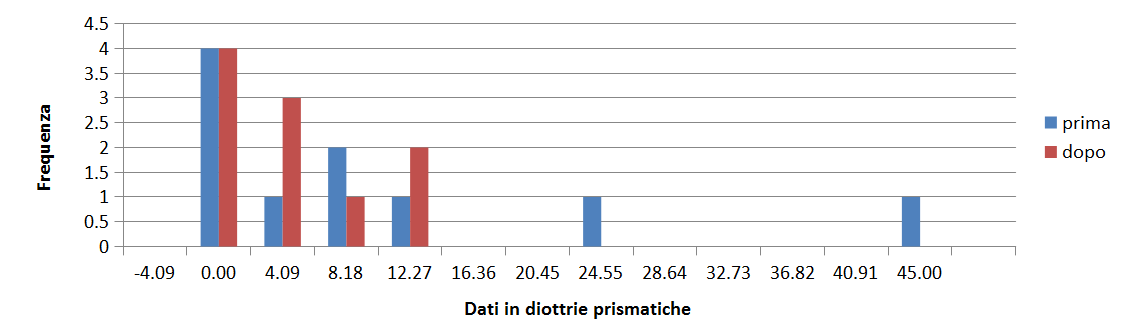
\includegraphics[scale=0.8]{source/grafici/COVER_TEST_7_TRATTATI_NUOVO.png}
	\caption[figure]{Grafico gruppo sperimentale per cover test 7: confronto tra prima visita e seconda visita}
	\label{fig:issuexample}
\end{figure}
 \begin{figure}[h!]
	\centering
	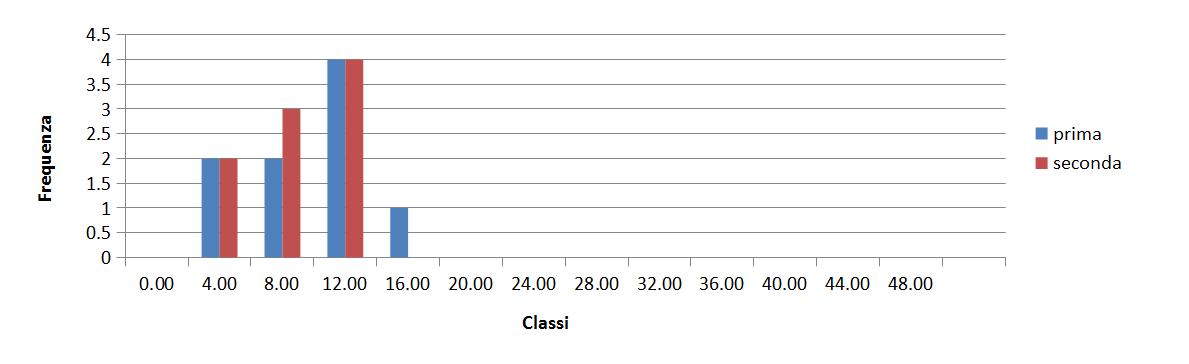
\includegraphics[scale=0.8]{source/grafici/cover_test_7_giustissimo_non_trattati.png}
	\caption[figure]{Grafico gruppo di controllo per cover test 7: confronto tra prima visita e seconda visita}
	\label{fig:issuexample}
\end{figure}

Il test di Wilcoxon fornisce un W-value di 17 con valore critico a 5. Il cambiamento non è quindi da considerarsi statisticamente significativo. Anche in questi istogrammi però è possibile notare lo spostamento delle colonne rosse verso sinistra, indicando che effettivamente un buon numero di soggetti (60\%) ha riscontrato un miglioramento dei valori, verificabile anche osservando i dati riportati in appendice. Stessa cosa non può essere detta per i soggetti appartenenti al gruppo di controllo, dove solo il 33,3% ha riportato un miglioramento dei dati.


\subsubsection{Cover test in posizione 8}

La posizione 8 corrisponde allo sguardo rivolto in alto a destra, stimolando i muscoli obliquo inferiore dell’occhio sinistro e il retto superiore dell’occhio destro. In questa posizione nel gruppo sperimentale 4 (40\%) soggetti ha riportato un miglioramento, 2 (20\%) sono rimasti invariati e 4 (40\%) sono peggiorati. Nel gruppo di controllo nessun (0\%) soggetto è migliorato, uno (11,1\%) è rimasto invariato e 8 (88,8\%) soggetti sono peggiorati. Come per il cover test 7 sono state riportate le tabelle dei valori medi e gli istogrammi rappresentanti i dati ricavati durante la prima e seconda visita.

%%%%%%%%%%%%%%%%%%
\begin{table}
\centering
\setlength\tabcolsep{4pt}
\begin{minipage}{0.48\textwidth}
\centering
\tablewidth=\textwidth

\begin{tabular}{|c|c|c|} \hline
{\textbf{}} & {\textbf{  \hspace{8pt}Prima\hspace{8pt} }} & {\textbf{ \hspace{8pt}Dopo\hspace{8pt}  }}\\ \hline
\textbf{Numeri dati} & 10 & 10 \\ 
\textbf{Media} & 14.10 & 9.60 \\  
\textbf{Dev. Std.} & 14.84 & 6.02 \\  
\textbf{Mediana} & 12.00 & 8.00 \\ 
\textbf{Moda} & 0.00 & 8.00 \\ 
\textbf{Errore Std.} & 15.74 & 6.28 \\ 
\hline
\end{tabular}
\caption{Dati gruppo sperimentale Cover test 8}

\label{tab:accuracy} 
\end{minipage}%
\hfill
\begin{minipage}{0.48\textwidth}
\centering

\begin{tabular}{|c|c|c|} \hline
{\textbf{}} & {\textbf{  \hspace{8pt}Prima\hspace{8pt} }} & {\textbf{ \hspace{8pt}Dopo\hspace{8pt}  }}\\ \hline
\textbf{Numeri dati} & 9 & 9 \\ 
\textbf{Media} & 10.00 & 15.89 \\  
\textbf{Dev. Std.} & 6.08 & 8.34 \\  
\textbf{Mediana} & 8.00 & 16.00 \\  
\textbf{Moda} & 8.00 & \textbackslash \\
\textbf{Errore Std.} & 6.17 & 8.92 \\
\hline
\end{tabular}
\caption{Dati gruppo di controllo Cover test 8}

 \label{tab:ompdiff} 
\end{minipage}
\end{table}
%%%%%%%%%%%%%%%%%%%%%
 \begin{figure}[h!]
	\centering
	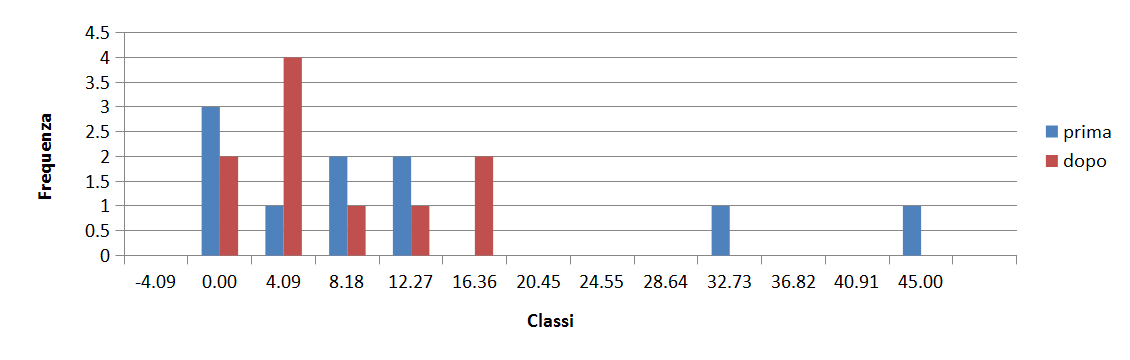
\includegraphics[scale=0.8]{source/grafici/cover_test_8_trattati_nuovo.png}
	\caption[figure]{Grafico gruppo sperimentale per Cover test 8: confronto tra prima e seconda valutazione}
	\label{fig:issuexample}
\end{figure}
 \begin{figure}[h!]
	\centering
	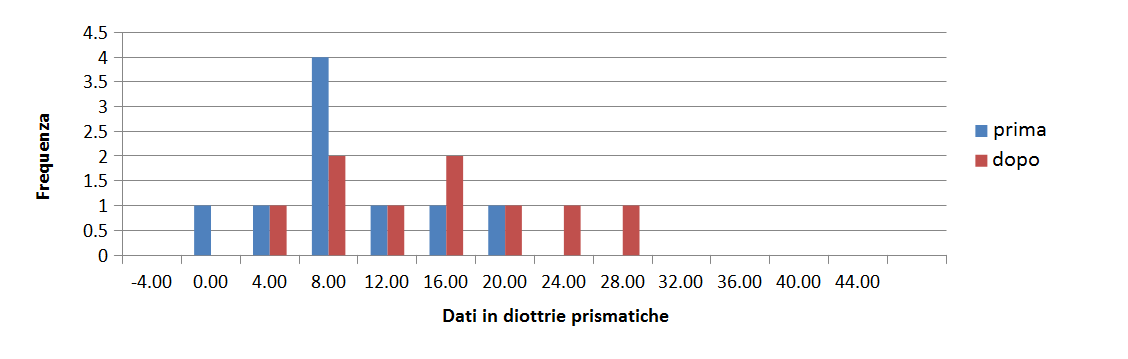
\includegraphics[scale=0.8]{source/grafici/cover_test_8_giustissimo_non_trattati.png}
	\caption[figure]{Grafico gruppo di controllo per Cover test 8: confronto tra prima e seconda valutazione}
	\label{fig:issuexample}
\end{figure}

Il test di Wilcoxon un W-value di 15 con un valore critico di 4. Il cambiamento risulta quindi non significativo. Confrontando i dati del gruppo sperimentale e il gruppo di controllo si nota come, a differenza dei precedenti test, non è possibile riscontrare il miglioramento nella maggior parte dei soggetti trattati, ma è interessante notare come il gruppo non sottoposto a trattamento sia per l’88,8% peggiorato. Anche gli istogrammi mostrano ancora lo spostamento dei dati della seconda visita verso valori inferiori. 


\subsubsection{Stereopsi vicino}

I valori della stereopsi vicino sono riportati in appendice. Nel gruppo sperimentale è stato possibile riscontrare un miglioramento in 6 soggetti (60\%), 4 soggetti (40\%) sono rimasti invariati e nessuno (0\%) è peggiorato. Nel gruppo di controllo sono migliorati 4 soggetti (44,4\%), rimasti invariati 4 soggetti (44,4\%) e uno (11,1\%) è peggiorato. Nelle tabelle sono riportati i valori medi. Sotto sono riportati gli istogrammi con il confronto tra prima e seconda valutazione in soggetti trattati e non trattati.

%%%%%%%%%%%%%%%%%%
\begin{table}
\centering
\setlength\tabcolsep{4pt}
\begin{minipage}{0.48\textwidth}
\centering
\tablewidth=\textwidth

\begin{tabular}{|c|c|c|} \hline
{\textbf{}} & {\textbf{  \hspace{8pt}Prima\hspace{8pt} }} & {\textbf{ \hspace{8pt}Dopo\hspace{8pt}  }}\\ \hline
\textbf{Numeri dati} & 10 & 10 \\ 
\textbf{Media} & 138.00 & 44.00 \\  
\textbf{Dev. Std.} & 146.20 & 12.65 \\  
\textbf{Mediana} & 70.00 & 40.00 \\ 
\textbf{Moda} & 40.00 & 40.00 \\ 
\textbf{Errore Std.} & 154.53 & 11.44 \\ 
\hline
\end{tabular}
\caption{Dati gruppo sperimentale Cover test 8}

\label{tab:accuracy} 
\end{minipage}%
\hfill
\begin{minipage}{0.48\textwidth}
\centering

\begin{tabular}{|c|c|c|} \hline
{\textbf{}} & {\textbf{  \hspace{8pt}Prima\hspace{8pt} }} & {\textbf{ \hspace{8pt}Dopo\hspace{8pt}  }}\\ \hline
\textbf{Numeri dati} & 9 & 9 \\ 
\textbf{Media} & 180.00 & 148.89 \\  
\textbf{Dev. Std.} & 172.55 & 153.33 \\  
\textbf{Mediana} & 50.00 & 40.00 \\  
\textbf{Moda} & 40.00 & 40.00 \\
\textbf{Errore Std.} & 154.99 & 147.63 \\
\hline
\end{tabular}
\caption{Dati gruppo di controllo Cover test 8}

 \label{tab:ompdiff} 
\end{minipage}
\end{table}
%%%%%%%%%%%%%%%%%%%%%
 \begin{figure}[h!]
	\centering
	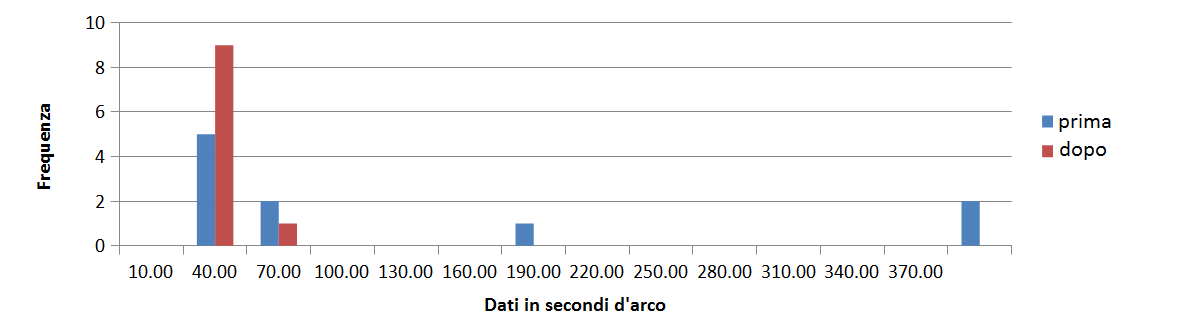
\includegraphics[scale=0.8]{source/grafici/STEREOPSI_VICINO_TRATTATI.png}
	\caption[figure]{Grafico gruppo sperimentale per la Stereopsi vicino: confronto tra prima e seconda valutazione}
	\label{fig:issuexample}
\end{figure}
 \begin{figure}[h!]
	\centering
	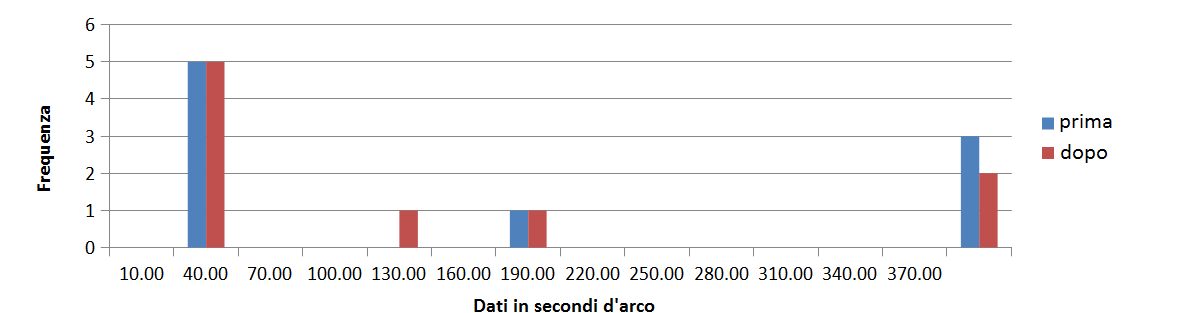
\includegraphics[scale=0.8]{source/grafici/STEREOPSI_VICINO_NON_TRATTATI.png}
	\caption[figure]{Grafico gruppo di controllo per la Stereopsi vicino: confronto tra prima e seconda valutazione}
	\label{fig:issuexample}
\end{figure}

Il test di Wilcoxon fornisce un W-value di 0 con valore critico a 0. Il cambiamento è quindi da considerarsi significativo. Infatti in questo test è evidente la presenza di un cambiamento anche negli istogrammi riportati e nei valori medi. Inoltre è possibile osservare come nel gruppo sottoposto al trattamento il 60\% dei soggetti abbia riscontrato un miglioramento che ha portato 9 soggetti su 10 a vedere tutti i cerchi in rilievo e nessuno sia peggiorato. 



\subsection{Analisi dei casi clinici}

Per concludere viene riportata la descrizione di due casi clinici maggiormente significativi dal punto di vista dei risultati ottenuti. Entrambi hanno effettuato il trattamento ma è stato applicato un differente impegno.
\\\ \\\
\textbf{Soggetto n°1: C.G. 14 anni, femmina}
\\\
Dopo la valutazione osteopatica-posturale, avvenuta il 6 settembre 2016, è stato possibile verificare che C.G. fosse affetta da deglutizione atipica con interposizione linguale e malocclusione in II classe dentale. È stata quindi inserita, per sua scelta, nel gruppo dei trattati e si è perciò sottoposta al trattamento logopedico-osteopatico per 3 mesi. Dall’analisi visiva effettuata il 15 settembre, prima del trattamento, e il 22 dicembre, dopo il trattamento, si sono ottenuti questi dati:

\begin{table}[H]
\begin{center}
\begin{tabular}{|c|c|c|} \hline
{\textbf{}} & {\textbf{Prima}} & {\textbf{Dopo}}\\ \hline
\textbf{Difetto refrattivo} & +0,50 D (entrambi gli occhi) & 0 D entrambi gli occhi \\ \hline
\textbf{Foria lontano} & 1 eso & 0.50 eso \\ \hline
\textbf{Stereopsi lontano} & 30" & 30" \\ \hline
\textbf{PPC dirito} & 16 cm & 3 cm \\ \hline
\textbf{PPC alto} & 20 cm & 5 cm \\ \hline
\textbf{PPC basso} & 15 cm & 3 cm\\ \hline
\textbf{Foria vicino alto} & 0.50 exo & 0.50 exo \\ \hline
\textbf{Foria vicino diritto} & 1 exo & 1 exo \\ \hline
\textbf{Foria vicino basso} & 1 exo & 1 exo \\ \hline
\textbf{CT 1} & 12 exo & 4 exo \\ \hline
\textbf{CT 2} & 14 exo & 8 exo \\ \hline
\textbf{CT 3} & 14 exo & 6 exo \\ \hline
\textbf{CT 4} & 0 & 4 exo \\ \hline
\textbf{CT 5} & 10 exo & 6 exo \\ \hline
\textbf{CT 6} & 10 exo & 4 exo \\ \hline
\textbf{CT 7} & 0 & 4 exo \\ \hline
\textbf{CT 8} & 13 exo & 8 exo \\ \hline
\textbf{CT 9} & 0 & 4 exo \\ \hline
\textbf{Ampiezza accomodativa OD} & 14 D (5 cm) & 16.60 D (13 cm)\\ \hline
\textbf{Ampiezza accomodativa OS} & 11 D (8 cm) & 14 D (8 cm)\\ \hline
\textbf{Ampiezza accomodativa OO} & 16.60 D (6 cm) & 16.60 D (11 cm) \\ \hline
\textbf{Stereopsi vicino} & 80" & 40" \\ \hline
\textbf{Disparità di fissazione} & 6.90 exo & 6.90 exo\\ \hline
\textbf{MEM OD} & 1.00 LAG  & 1.25 LAG \\ \hline
\textbf{MEM OS} & 1.25 LAG & 1.25 LAG\\ \hline

\hline
\end{tabular}
\end{center}
\caption{Dati valutazione di C.G.}
\end{table}

I dati rivelano la presenza di disfunzioni del sistema visivo, soprattutto riguardo il punto prossimo di convergenza, il cover test nelle 9 posizioni di sguardo, la stereopsi vicino e la disparità di fissazione. Si potrebbe ipotizzare un alterato utilizzo dei muscoli estrinseci dell’occhio per lo scompenso causato dalla deglutizione atipica e dalla malocclusione. Presenta inoltre una leggera ipermetropia a entrambi gli occhi corretta con lenti oftalmiche. C.G. ha effettuato con costanza gli esercizi proposti dalla logopedista e si è presentata ogni settimana all’ambulatorio per il trattamento osteopatico. È stata rivalutata il 22 dicembre, dopo 3 mesi e la situazione è notevolmente migliorata. Il punto prossimo di convergenza si è avvicinato notevolmente e anche i valori del cover test si sono abbassati. Complessivamente il soggetto ha riferito di non aver faticato nello svolgimento dei testi e di sentirsi più stabile anche dal punto di vista della postura. Si suppone quindi che sia migliorata la stabilità del sistema visivo del soggetto, dal momento che migliora la capacità di mantenere singola la mira durante il PPC e questo può aver portato ad una maggiore consapevolezza dello spazio e quindi al miglioramento del valore della stereopsi.
\\\ \\\
\textbf{Soggetto n°2: V.M. 22 anni, femmina}
\\\
Un caso molto interessante è quello di V.M. di 22 anni. Il soggetto si presenta dall’osteopata per difficoltà di equilibrio che non le permettevano di rimanere a lungo in piedi. Dall’analisi osteopatica-posturale è emersa la primarietà dell’apparato stomatognatico per la presenza di deglutizione atipica. È stata quindi sottoposta al trattamento logopedico-osteopatico in seguito alla prima visita optometrica avvenuta il 15 settembre 2016. È stata successivamente rivalutata il 5 gennaio 2017 dopo un trattamento di circa 3 mesi. Di seguito è riportato ciò che è stato rilevato:

\begin{table}[H]
\begin{center}
\begin{tabular}{|c|c|c|} \hline
{\textbf{}} & {\textbf{Prima}} & {\textbf{Dopo}}\\ \hline
\textbf{Difetto refrattivo} & OD: +0,25 D; OS: -1,75 D & OD: 0 D; OS: -1,25 D \\ \hline
\textbf{Foria lontano} & 0 & 0\\ \hline
\textbf{Stereopsi lontano} & ASSENTE & ASSENTE \\ \hline
\textbf{PPC dirito} & 8 cm & 9 cm \\ \hline
\textbf{PPC alto} & 4 cm & 13 cm \\ \hline
\textbf{PPC basso} & 1 cm & 4 cm \\ \hline
\textbf{Foria vicino alto} & 0 & 0.50 exo \\ \hline
\textbf{Foria vicino diritto} & 0.50 exo & 0 \\ \hline
\textbf{Foria vicino basso} & 2 exo & 1 exo \\ \hline
\textbf{CT 1} & 12 exo & 6 exo \\ \hline
\textbf{CT 2} & 20 exo & 14 exo \\ \hline
\textbf{CT 3} & 0 exo & 2 exo \\ \hline
\textbf{CT 4} & 9 exo & 4 exo \\ \hline
\textbf{CT 5} & 20 exo & 8 exo \\ \hline
\textbf{CT 6} & 8 exo & 0 \\ \hline
\textbf{CT 7} & 9 exo & 6 exo \\ \hline
\textbf{CT 8} & 0 & 6 exo \\ \hline
\textbf{CT 9} & 0 & 4 exo \\ \hline
\textbf{Ampiezza accomodativa OD} & 20 D & 7.70 D \\ \hline
\textbf{Ampiezza accomodativa OS} & 12.50 D & 12.50 D \\ \hline
\textbf{Ampiezza accomodativa OO} & 16.60 D & 9 D \\ \hline
\textbf{Stereopsi vicino} & 400" & 40" \\ \hline
\textbf{Disparità di fissazione} & SOPPRESSIONE OD & 13.70 exo \\ \hline
\textbf{MEM OD} & 1.50 LAG & 2.25 LAG \\ \hline
\textbf{MEM OS} & 0.25 LEAD & 0.25 LEAD \\ \hline

\hline
\end{tabular}
\end{center}
\caption{Dati valutazione di V.M.}
\end{table}

In questo caso è interessante osservare come i dati prima del trattamento evidenziassero un’instabilità della binocularità data dalla soppressione dell’occhio destro. Sono anche alterati i valori del cover test, i quali sono migliorati nella seconda visita. V.M. ha effettuato con minore costanza l’esercizio logopedico e le sedute osteopatiche rispetto al soggetto n°1. Nonostante questo ha mostrato dei miglioramenti soprattutto dal punto di vista dell’equilibrio. V.M. infatti non lamenta più perdite di equilibrio ed ha svolto i test optometrici della seconda visita con maggiore facilità rispetto alla prima. La difficoltà di equilibrio la si può riscontrare anche a livello oculare, infatti la binocularità risultava compromessa. Nella seconda valutazione il cambiamento riguarda il test della stereopsi vicino e della disparità di fissazione, i quali forniscono informazioni su come viene utilizzata la binocularità. Si suppone che la maggior stabilità dei muscoli oculari, rilevata con il cover test, abbia portato a un miglior utilizzo degli stessi e quindi una migliore stabilità binoculare.

\section{Conclusioni}

A conclusione della ricerca e dell’analisi statistica dei dati è stato possibile osservare che il cambiamento non è risultato statisticamente significativo per la maggior parte dei test effettuati.

Analizzando i valori medi è stato possibile riscontrare un miglioramento nei test di Punto Prossimo di Convergenza, Cover test (a destra e in alto a destra) e Stereopsi vicino. Tra questi è stato rilevato un cambiamento da considerarsi statisticamente significativo solo nel test della Stereopsi vicino. Il sistema visivo potrebbe infatti aver trovato una migliore stabilità a seguito del trattamento all’apparato stomatognatico, permettendo una maggiore consapevolezza dello spazio e quindi un miglioramento della percezione della profondità. Sicuramente il miglioramento della stereopsi sarà dovuto al miglioramento della binocularità del soggetto e quindi dovrebbe essere legato alle altre funzioni. Quindi nonostante non sia evidenziato un cambiamento statisticamente significativo, un miglioramento delle altre funzioni dovrebbe aver influenzato il rientro dei valori della stereopsi nella normalità.
 
A causa dei pochi dati non è possibile fornire informazioni statisticamente attendibili ed è aperta l’ipotesi che si possa trattare di un cambiamento casuale, ma, dal confronto dei risultati del gruppo sperimentale e del gruppo di controllo, è possibile anche ipotizzare l’efficacia del trattamento logopedico-osteopatico su soggetti con primarietà linguale. Il miglioramento delle disfunzioni dell’apparato stomatognatico ha permesso al sistema visivo di trovare una nuova stabilizzazione, quindi è probabile che se fosse stata effettuata una terza valutazione a distanza di altri mesi di trattamento, si sarebbe potuto osservare un cambiamento maggiormente significativo anche in altre funzioni del sistema visivo. Pertanto questa ricerca può essere considerata come un punto di partenza per indagare quali sono le funzioni visive che sono maggiormente legate all’apparato stomatognatico.  Infatti complessivamente 5 soggetti trattati su 10 hanno riportato maggiore stabilità delle funzionalità del sistema visivo, con un miglioramento complessivo dei valori. 

Nella ricerca sono state riscontrate diverse difficoltà e diversi limiti:
\begin{itemize}
 \itemsep-0.5em
 \item[--]Il campionamento era molto selettivo, quindi è stato difficile riuscire ad includere un maggior numero di soggetti nel tempo avuto a disposizione, dal momento che molte persone inizialmente incluse, sono venuti meno all’impegno o hanno deciso di non continuare la partecipazione della ricerca.
 \item[--]La riuscita della ricerca dipendeva fortemente dall’impegno dei soggetti, i quali sono stati seguiti dalla laureanda e dalla logopedista attraverso la compilazione di un diario a casa e attraverso appuntamenti in ambulatorio. Il limite è stato doversi affidare al loro impegno.
 \item[--]È necessario tenere conto delle condizioni di salute del soggetto al momento della valutazione. Spesso è stata effettuata dopo la scuola o dopo il lavoro, quando il soggetto aveva già applicato uno sforzo visivo, il quale potrebbe aver alterato i risultati.
\end{itemize}

Per ulteriori sviluppi futuri sarebbe interessante sottoporre i soggetti ad un questionario riguardo la loro condizione di salute prima di ogni valutazione optometrica, per essere sicuri che le condizioni di salute siano le stesse e quindi si possano rendere i dati più realistici. Sarebbe interessante anche approfondire il cambiamento del punto prossimo di convergenza utilizzando un campione più ampio per comprendere quanto la disfunzione della deglutizione possa influire sulla convergenza; infatti si potrebbe effettuare un confronto con quanto riportato in letteratura, dove si registra un cambiamento della convergenza trattando le mal occlusioni dentali. 

Nonostante le difficoltà riscontrate, essa può essere un buon punto di partenza per un ulteriore approfondimento su quali sono le funzioni visive maggiormente connesse all’apparato stomatognatico e che quindi possono essere alterate da una disfunzione di esso. La ricerca potrebbe essere continuata e quindi si potrebbe costituire un campione più grande in modo da rendere più attendibili le analisi statistiche. Il lavoro effettuato ha mostrato comunque risultati soddisfacenti considerando i pochi soggetti coinvolti e costituisce un esempio di lavoro multidisciplinare. Infatti in quanto optometristi dovremmo ricordare che gli occhi del soggetto che valutiamo fanno parte di un sistema molto più ampio e complesso e quindi una disfunzione del sistema visivo potrebbe derivare da un mal funzionamento di altri sistemi. Pertanto non sono sempre le lenti oftalmiche che permettono un miglioramento delle funzioni visive, spesso è  un trattamento eseguito con impegno e costanza in un distretto del corpo che può portare a importanti miglioramenti su tutto il sistema posturale, compreso il sistema visivo.

É un buon punto di partenza per poter fare in modo che chi farà una ricerca di questo tipo non incorrerà negli stessi errori